
\documentclass[a4paper,11pt]{article}%,twocolumn
%% packages

\usepackage{blindtext} % needed for creating dummy text passages
%\usepackage{ngerman} % needed for German default language
\usepackage{amsmath} % needed for command eqref
\usepackage{amssymb} % needed for math fonts
\usepackage[colorlinks=true,breaklinks]{hyperref} % needed for creating hyperlinks in the document, the option colorlinks=true gets rid of the awful boxes, breaklinks breaks lonkg links (list of figures), and ngerman sets everything for german as default hyperlinks language
\usepackage[hyphenbreaks]{breakurl} % ben�tigt f�r das Brechen von URLs in Literaturreferenzen, hyphenbreaks auch bei links, die �ber eine Seite gehen (mit hyphenation).
\usepackage{xcolor}
\definecolor{c1}{rgb}{0,0,1} % blue
\definecolor{c2}{rgb}{0,0.3,0.9} % light blue
\definecolor{c3}{rgb}{0.3,0,0.9} % red blue
\hypersetup{
    linkcolor={c1}, % internal links
    citecolor={c2}, % citations
    urlcolor={c3} % external links/urls
}
%\usepackage{cite} % needed for cite
\usepackage[square,authoryear]{natbib} % needed for cite and abbrvnat bibliography style
\usepackage[nottoc]{tocbibind} % needed for displaying bibliography and other in the table of contents
\usepackage{graphicx} % needed for \includegraphics 
\usepackage{longtable} % needed for long tables over pages
\usepackage{bigstrut} % needed for the command \bigstrut
\usepackage{enumerate} % needed for some options in enumerate
%\usepackage{todonotes} % needed for todos
\usepackage{makeidx} % needed for creating an index
\makeindex
\usepackage{gensymb}
\usepackage{url}
\usepackage{psfrag}
\usepackage{multirow}
\usepackage{subfigure}
%% page settings

\usepackage[top=20mm, bottom=20mm,left=15mm,right=15mm]{geometry} % needed for page border settings
\parindent=0mm % for space of first line of new text block
\sloppy % for writing with hyphenless justification (tries to)
\hyphenation{} % use hyphenation of tolerance parametershttp://www.jr-x.de/publikationen/latex/tipps/zeilenumbruch.html
\hyphenpenalty=10000
\exhyphenpenalty=10000
\usepackage{fancyhdr} % needed for head and foot options
%% my macros

%% Text fomats
\newcommand{\tbi}[1]{\textbf{\textit{#1}}}

%% Math fonts
\newcommand{\bbA}{\mathbb{A}}
\newcommand{\bbB}{\mathbb{B}}
\newcommand{\bbC}{\mathbb{C}}
\newcommand{\bbD}{\mathbb{D}}
\newcommand{\bbE}{\mathbb{E}}
\newcommand{\bbF}{\mathbb{F}}
\newcommand{\bbG}{\mathbb{G}}
\newcommand{\bbH}{\mathbb{H}}
\newcommand{\bbI}{\mathbb{I}}
\newcommand{\bbJ}{\mathbb{J}}
\newcommand{\bbK}{\mathbb{K}}
\newcommand{\bbL}{\mathbb{L}}
\newcommand{\bbM}{\mathbb{M}}
\newcommand{\bbN}{\mathbb{N}}
\newcommand{\bbO}{\mathbb{O}}
\newcommand{\bbP}{\mathbb{P}}
\newcommand{\bbQ}{\mathbb{Q}}
\newcommand{\bbR}{\mathbb{R}}
\newcommand{\bbS}{\mathbb{S}}
\newcommand{\bbT}{\mathbb{T}}
\newcommand{\bbU}{\mathbb{U}}
\newcommand{\bbV}{\mathbb{V}}
\newcommand{\bbW}{\mathbb{W}}
\newcommand{\bbX}{\mathbb{X}}
\newcommand{\bbY}{\mathbb{Y}}
\newcommand{\bbZ}{\mathbb{Z}}


% Define colors
\definecolor{codegreen}{rgb}{0,0.6,0}
\definecolor{codegray}{rgb}{0.5,0.5,0.5}
\definecolor{codepurple}{rgb}{0.58,0,0.82}
\definecolor{backcolour}{rgb}{0.95,0.95,0.92}
% Setup the listings package
\lstset{
    backgroundcolor=\color{backcolour},   
    commentstyle=\color{codegreen},
    keywordstyle=\color{magenta},
    numberstyle=\tiny\color{codegray},
    stringstyle=\color{codepurple},
    basicstyle=\footnotesize,
    breakatwhitespace=false,         
    breaklines=true,                 
    captionpos=b,                    
    keepspaces=true,                 
    numbers=left,                    
    numbersep=5pt,                  
    showspaces=false,                
    showstringspaces=false,
    showtabs=false,                  
    tabsize=2
}



\begin{document}
\begin{titlepage}
\center % Center everything on the page

%-------------------------------------------------------------------------------------
%	HEADING SECTIONS
%------------------------------------------------------------------------------------
\textbf{\large Department of Electrical and Computer Engineering}\\[0.5cm]
\textbf{\Large University of Colorado at Boulder}\\[1cm]
\textbf{\large ECEN5730 - Practical PCB design}\\[2cm]

\includegraphics[width=0.3\textwidth]{figures/cu}\\[2cm] 

	
%-------------------------------------------------------------------------------------
%	TITLE SECTION
%------------------------------------------------------------------------------------

\textbf{\Huge Board Good Layout/Bad Layout }\\[0.2cm]

\textbf{\Large Report}\\[2cm]
\vspace{1.5cm}
\begin{figure}[H]
	\centering
	
\includegraphics[scale=0.2]{figures/qr_download.png}
	\label{555_schematic}
\end{figure}\vspace{1.5cm}


%----------------------------------------------------------------------------------------
%	MEMBERS SECTION
%----------------------------------------------------------------------------------------


\vfill

\textbf{\large Submitted by}

{\large Parth Thakkar}\\[0.5cm]




%----------------------------------------------------------------------------------------
%	DATE SECTION
%----------------------------------------------------------------------------------------

\textbf{\large Submitted on}\\
\textbf{\Large \today} % Date, change the \today to a set date if you want to be precise

%----------------------------------------------------------------------------------------

\vfill % Fill the rest of the page with whitespace

\end{titlepage}

\pagebreak

\tableofcontents
\listoffigures
\listoftables
\vfill
\begin{center}
	\textbf{\textit{*PDF is clickable}}
\end{center}

\pagebreak

\section{Objective / Purpose of Lab}

\begin{itemize}
	\item To distinguish between the methodologies of differential and single-ended signal measurements, pinpointing their individual merits and drawbacks. This objective was achieved through the utilization of a TMP36 temperature sensor and an ADS1115 analog-to-digital converter (ADC).

	\item To examine the influence of ground noise on the integrity of signals for both differential and single-ended setups.
	
	\item ADS1115 module for data capture through the I2C communication protocol. This included adjustments in gain settings, sample rates, and addressing configurations, aimed at bolstering our proficiency in employing digital communications for sensor data gathering and ADC adjustments to achieve heightened measurement precision.
	
	\item To explore the effectiveness of averaging in diminishing noise within signal measurements. This was executed by developing software routines for collecting, averaging, and evaluating multiple ADC readings.

	
	\item To implement differential measurement strategies for achieving improved signal clarity in scenarios affected by ground noise, underscoring the practical advantages of differential signaling in electronic circuit design.\\
	
	
	\begin{figure}[!h]
		\centering
		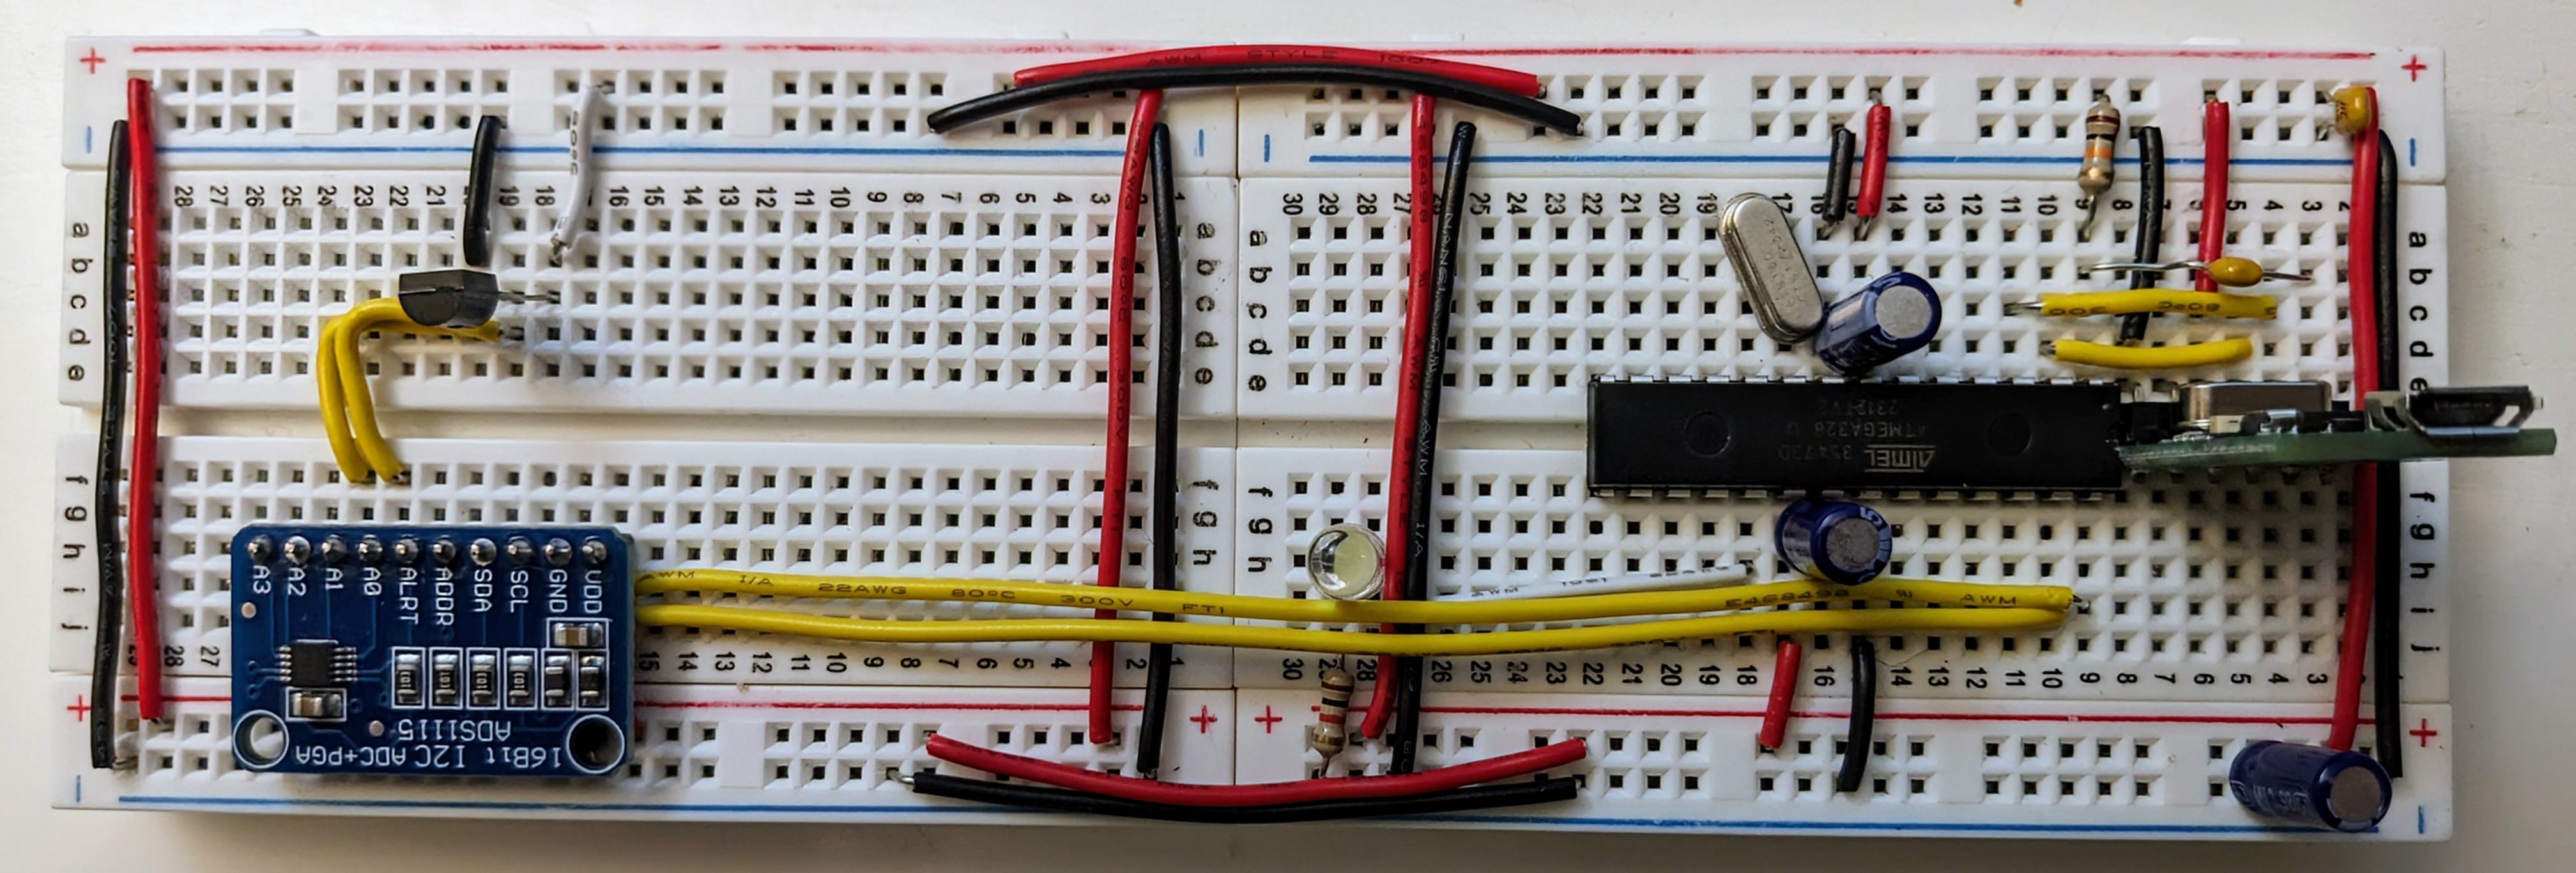
\includegraphics[scale=0.12]{figures/breadboard.jpg}
		\caption{PCB}

	\end{figure}
	
\end{itemize}

\section{Component listing}


\begin{table}[H]
	\centering 
	\begin{tabular}{|c|l|}
		\hline
		&\textbf{Component Name}\\\hline
		
		&\\
		1&Digital Multimeter (DMM)\\
		2&ADS1115 ADC sensor\\
		2&TMP36 Temperature Sensor\\
		2&Solderless Breadboard\\
		2&Function Generator \\
\hline\hline
	\end{tabular}
	\caption{Component list}
	\label{filterspecs}
\end{table}





\section{Explanation}


\textbf{Single-Ended Signaling}
Single-ended signaling is a method of measuring or transmitting information where the signal is represented as a voltage relative to a common ground. In this setup, each signal requires one wire plus a ground connection. The simplicity of single-ended signaling makes it appealing for many applications; however, it is inherently more susceptible to noise. Noise can be introduced into the system from various sources, including electromagnetic interference (EMI) from nearby electrical devices or inherent noise within the circuit itself. Since the signal is measured against a common ground, any fluctuation in the ground voltage due to noise directly affects the accuracy of the signal measurement.

\textbf{Differential Signaling}
Differential signaling, in contrast, utilizes pairs of wires to transmit signals, with each wire carrying a signal that is the inverse of the other. The actual signal is the difference in voltage between these two wires, which effectively doubles the signal voltage and cancels out common-mode noise. This method is inherently more resistant to external noise because any noise that is picked up on the signal path is likely to be common to both lines and is thus canceled out when the difference is taken. Differential signaling is particularly advantageous in environments with significant electrical noise or over long transmission distances where signal integrity is crucial.

\textbf{ADS1115 and Differential Measurement Support}
The ADS1115 module is a precision, low-power, 16-bit analog-to-digital converter (ADC) that offers high-resolution measurements and supports both single-ended and differential inputs. This capability makes the ADS1115 an excellent tool for exploring the differences between single-ended and differential measurements in a lab setting. The ADS1115 features four input channels, which can be configured either as four single-ended inputs or two differential pairs, providing flexibility in measurement setups.

The module communicates with a microcontroller, such as an Arduino, via the I2C protocol, allowing for easy integration into a variety of projects. For differential measurements, the ADS1115 can compare the voltage between two inputs (e.g., AIN0 and AIN1 for one differential pair) and convert this voltage difference into a digital value. This feature is particularly useful in experiments designed to demonstrate the efficacy of differential signaling in reducing the impact of noise on signal measurements.


\section{Procedure}

\textbf{Arduino IDE Configuration}
Launch the Arduino IDE on your computer.
Install the Adafruit ADS1X15 library (if it's not already installed) by going to Sketch > Include Library > Manage Libraries…, then search for "Adafruit ADS1X15" and click "Install".


\textbf{Wiring the Circuit}
\begin{enumerate}
	\item Power Connections
	Connect the Arduino 5V and GND to the solderless breadboard's power rails. Use red wires for 5V and black wires for GND to maintain color consistency.
	\item TMP36 Sensor Wiring
	Place the TMP36 on the breadboard.
	Connect its left pin (facing the flat part towards you) to 5V, the middle pin to an unused row on the breadboard (for connection to the ADS1115 later), and the right pin to GND.
	\item ADS1115 Module Connections
	\begin{enumerate}
		\item Solder the header pins to the ADS1115 module if needed.
		\item Connect the module's VDD to 5V and GND to ground on the breadboard.
		\item Connect SCL to Arduino's A5 and SDA to A4.
		\item For differential measurements, connect AIN0 to the TMP36 middle pin and AIN1 to the TMP36 right pin.
		\item For single-ended measurements, connect AIN0 to the TMP36 middle pin.
	\end{enumerate}
	\item Connect the Arduino to your computer with a USB cable.
	
\end{enumerate}


Programming the Arduino
\begin{enumerate}
	\item Load the Sketch\\
	Open a new sketch in the Arduino IDE.
	At the beginning, include the Adafruit ADS1X15 library with \#include <Adafruit\_ADS1015.h>.
	\item Initialize the ADS1115\\
	In the setup() function, initialize the ADS1115 with ads.begin();.
	Set the gain as necessary using ads.setGain(GAIN\_TWOTHIRDS); for TMP36 voltage readings.
	\item Reading data\\
	\begin{itemize}
		\item For differential readings, use ads.readADC\_Differential\_0\_1(); in the loop() function.
		\item For single-ended readings, use ads.readADC\_SingleEnded(0); in the loop() function.
		\item Convert the raw data to voltage by applying the correct scale factor based on your gain setting.
	\end{itemize}
	\item 
	Serial Output\\
	Print the voltage readings to the Serial Monitor for observation in both differential and single-ended setups.
	
	\item Introducing Ground Noise \\
	To simulate ground noise, carefully inject a low-frequency signal into the ground path between the TMP36 and ADS1115 using a function generator.
\end{enumerate}


\section{Code}

\begin{lstlisting}[language=C]
	#include <Adafruit_ADS1X15.h>
	#include <Wire.h>
	Adafruit_ADS1115 ads;
	// instantiates the object
	float mV_per_ADU;
	long n_operations = 100;
	long iTimer0_usec;
	long iDummy;
	float Time_X_usec;
	void setup() {
	Serial.begin(1000000);
	delay(1000);                  //lets the serial port get initialized
	ads.begin(0x48);              //default address with addr pin connected to gnd
	ads.setGain(GAIN_TWOTHIRDS);  // 2/3x gain +/- 6.144V 1 bit = 3mV
	mV_per_ADU = 0.1875;          //for ADS1115
	}
	void loop() {
	//Serial.println(ads.readADC_SingleEnded(0)*mV_per_ADU);
	iTimer0_usec = micros();
	for (int i = 1; i <= n_operations; i++) {
		iDummy = ads.readADC_SingleEnded(0);
	}
	Time_X_usec = (micros() - iTimer0_usec) / (n_operations * 1.0);
		Serial.print(" Xtime_usec: ");
	Serial.print(Time_X_usec, 3);
	Serial.print(" Frequency (Hz): ");
	Serial.print(1e6 / (Time_X_usec), 3);
	Serial.println();
	}
\end{lstlisting}

Output :
\begin{figure}[!h]
	\centering
	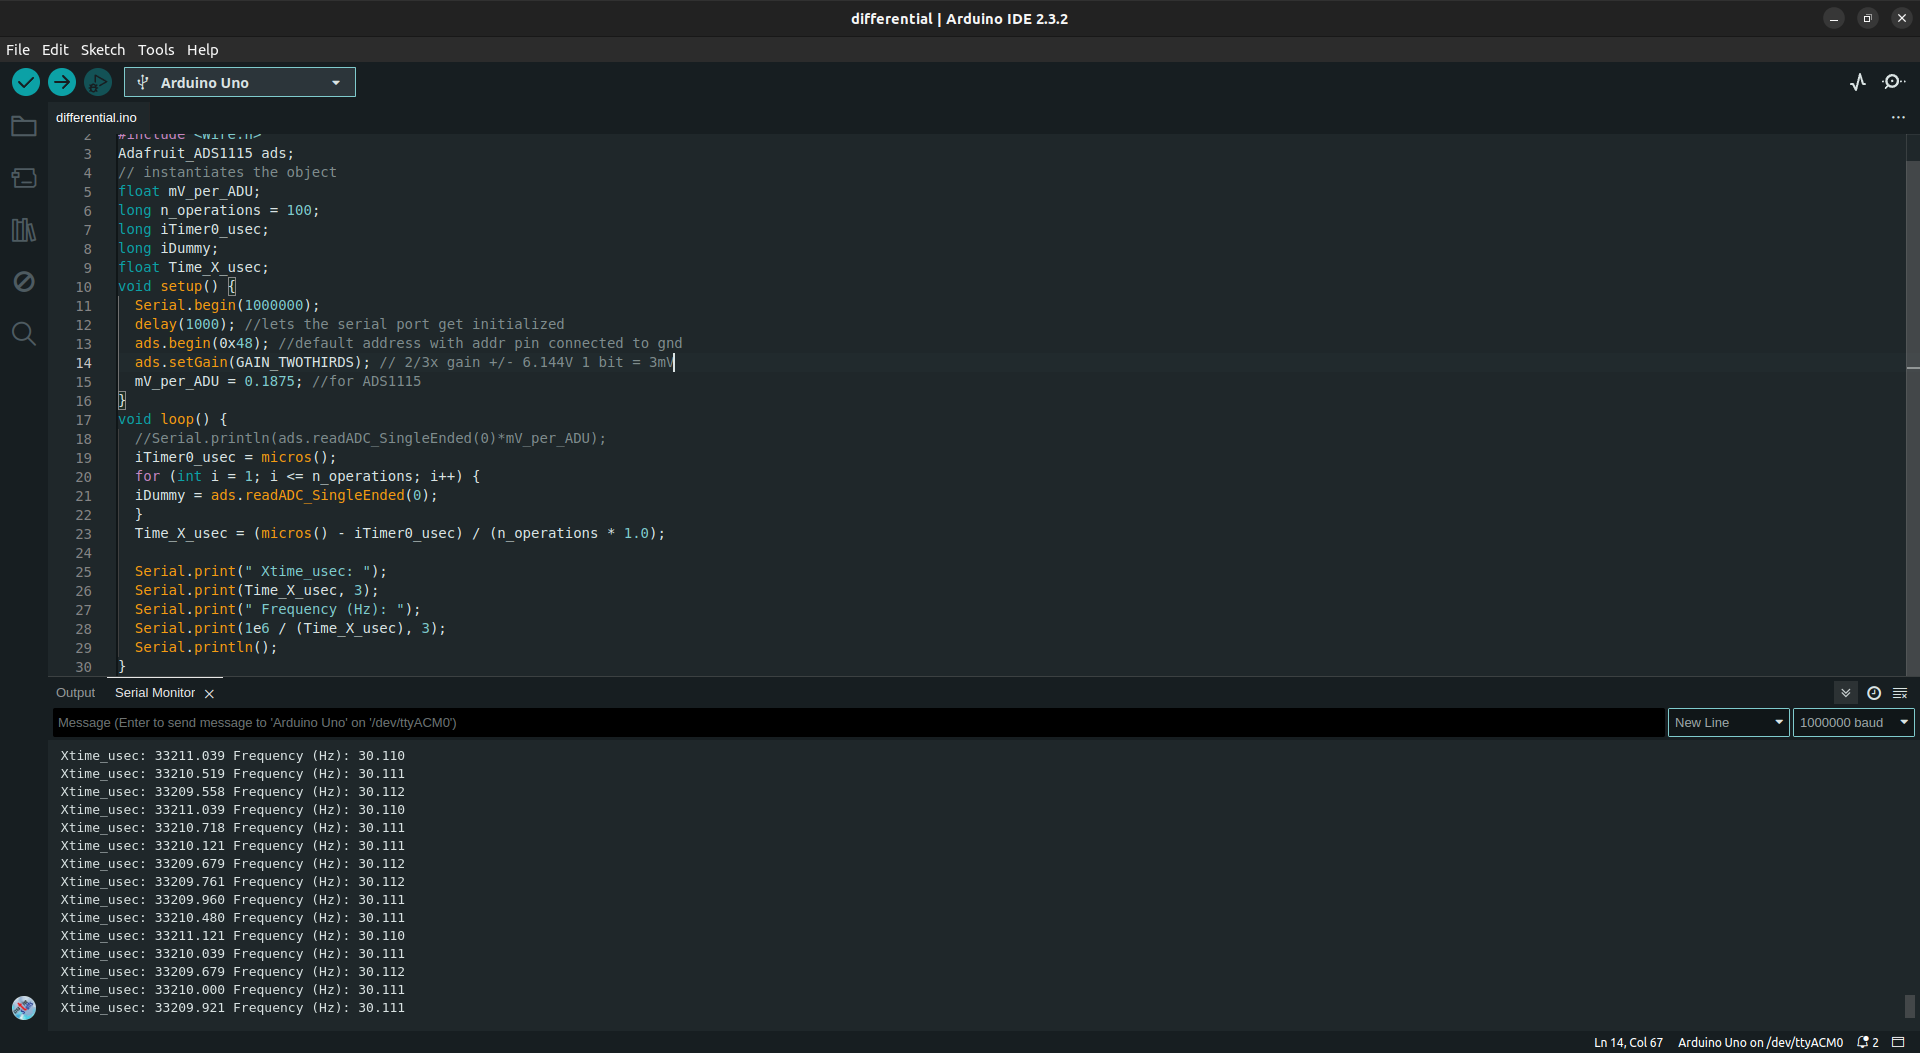
\includegraphics[scale=0.25]{figures/readings.png}
	\caption{Frequency}
\end{figure}



\begin{lstlisting}[language=C]
	#include <Wire.h>
	#include <Adafruit_ADS1X15.h>
	Adafruit_ADS1115 ads;      /* Use this for the 16-bit version */
	int iTime_ave_msec = 100;  //averaging time per point
	long iTime_stop_msec;
	int iCounter1 = 0;  //used in counting number of points
	float V_diff_mV;
	//used for diff voltage
	float V_SE_mV;
	// used for SE measurement
	void setup(void) {
	Serial.begin(2000000);

	ads.setGain(GAIN_FOUR);  // 4x gain

	// ads.setGain(GAIN_SIXTEEN);
	// 16x gain +/- 0.256V 1 bit = 0.125mV 0.0078125mV
	ads.begin();  //with the ADR pin set to gnd.
	ads.setDataRate(RATE_ADS1115_860SPS);
	}
	void loop(void) {
	V_diff_mV = 0.0;
	V_SE_mV = 0.0;
	iCounter1 = 0;
	iTime_stop_msec = micros() / 1000 + iTime_ave_msec;
	while (micros() / 1000 <= iTime_stop_msec) {
		V_diff_mV = V_diff_mV + ads.readADC_Differential_0_1() * 0.0312;
		V_SE_mV = V_SE_mV + ads.readADC_SingleEnded(0) * 0.0312;
		iCounter1++;
	}
	V_diff_mV = V_diff_mV / iCounter1;
	V_SE_mV = V_SE_mV / iCounter1;
	Serial.print(720);
	Serial.print(", ");
	Serial.print(760);
	Serial.print(", ");
	Serial.print(V_diff_mV);
	Serial.print(", ");
	Serial.println(V_SE_mV);
	}

\end{lstlisting}





\section{Measurement}



Results
Without Function Generator Noise: The baseline measurements showed a higher SNR in the differential configuration compared to the single-ended setup, indicating lower noise levels when differential signaling was used.

Here we don't see much noise while there is no noise in the ground.
\begin{lstlisting}[language=C]
	720, 760, 738.42, 733.62
	720, 760, 739.49, 734.14
	720, 760, 737.29, 736.56
	720, 760, 738.19, 734.63
	720, 760, 738.62, 736.36
	720, 760, 737.39, 738.43
	720, 760, 738.41, 741.68
	720, 760, 739.15, 743.68
	720, 760, 740.51, 743.33
\end{lstlisting}

With Function Generator Noise: The introduction of noise through the function generator significantly reduced the SNR in the single-ended configuration, demonstrating its susceptibility to external noise. Conversely, the differential configuration maintained a relatively high SNR, When we added noise ( Sine wave of 0.1 Hz at 10V peak to peak we got this kind of signal)
\begin{figure}[!h]
	\centering
	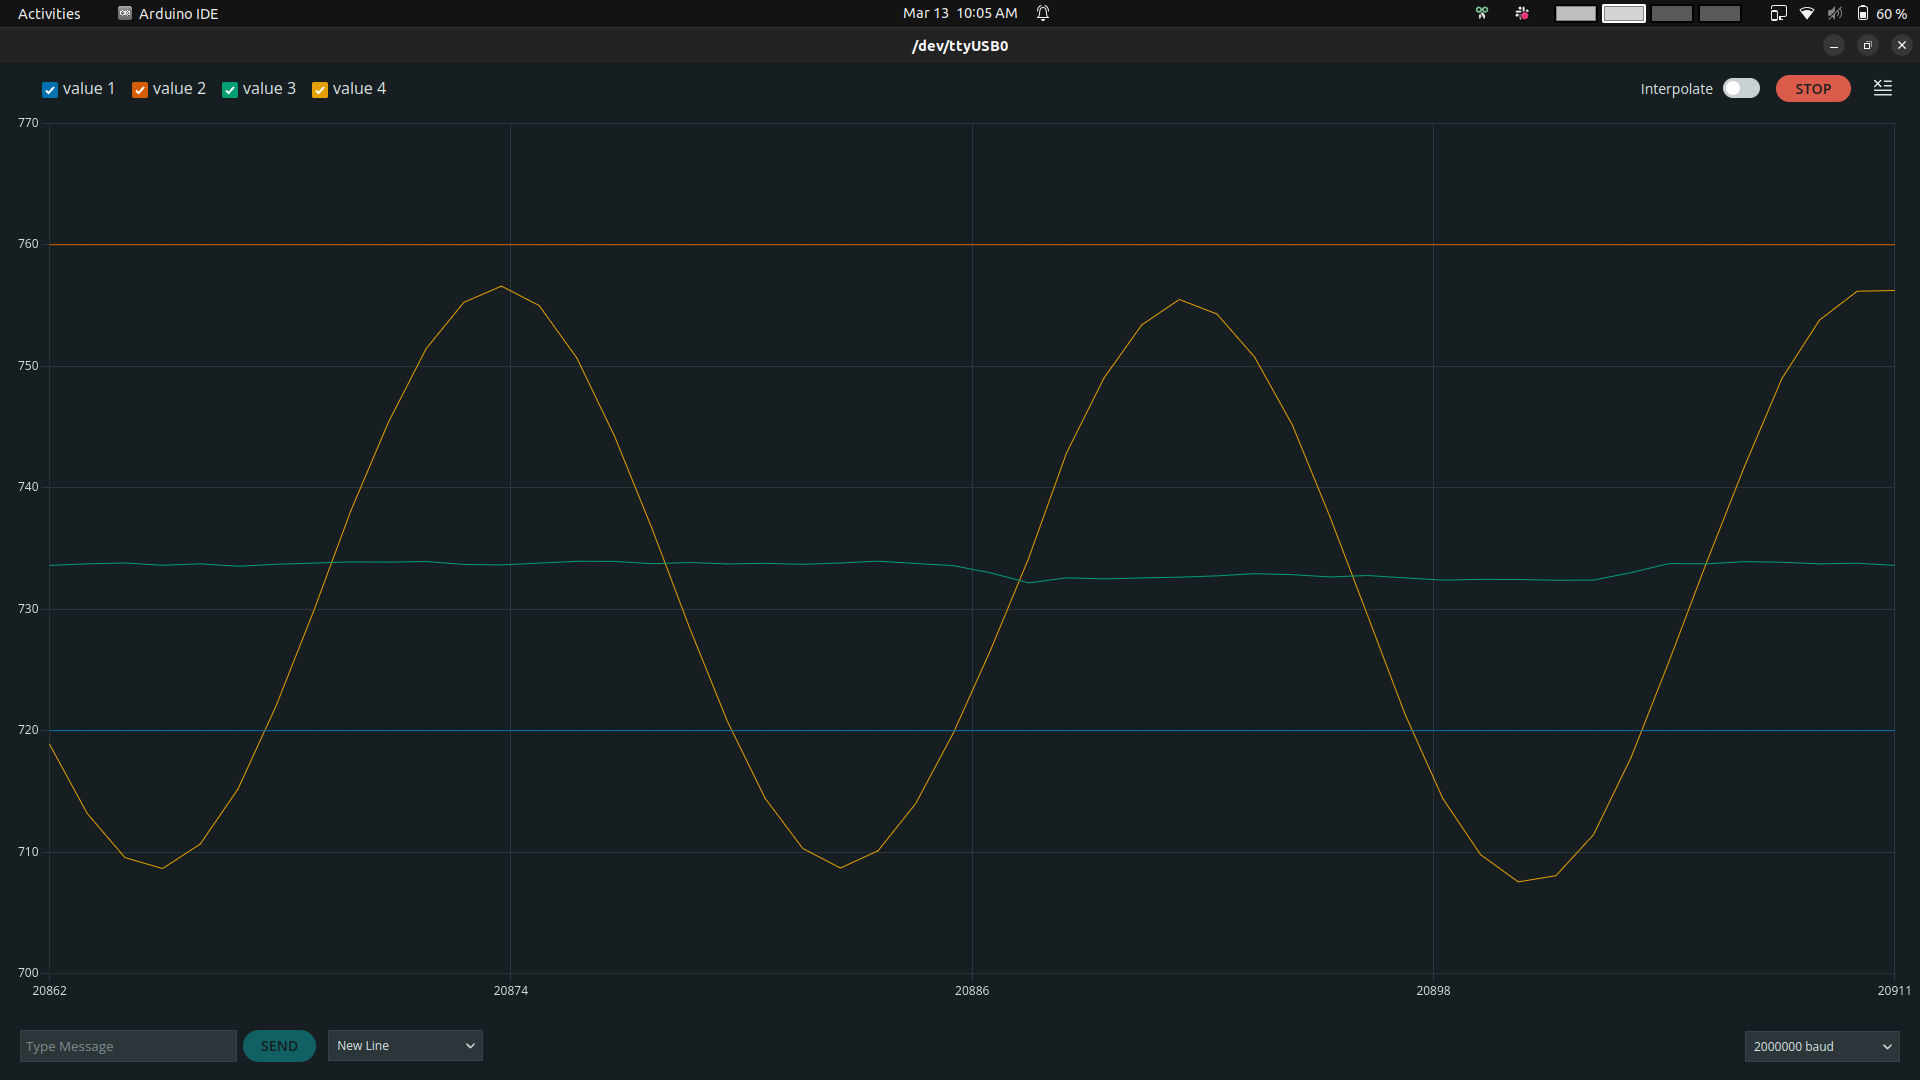
\includegraphics[scale=0.24]{figures/differential.png}
	\caption{Differential reading}

\end{figure}

\section{Learnings and Observation}
\begin{enumerate}
	\item In our lab, we looked at how outside noise, especially the kind made by a function generator, can affect the signals coming from a TMP36 temperature sensor. This test showed us that electronic signals are really sensitive to outside disturbances. We saw that noise could really lower the quality of our signal measurements, making our data less accurate and reliable.

	\item We also found out that using differential signaling is much better for dealing with noise than the single-ended method. When we compared the two, the differential setup was much better at ignoring the noise that was the same in both signals. This makes differential signaling a better choice in places with a lot of noise or when it's really important to keep the signal clear.
	
	\item The lab also made it clear how important it is to design and lay out your circuit carefully to keep noise out. It showed how choosing the right way to measure things and how you connect your wires can make your signal clearer.
	
	\item Getting to work directly with the ADS1115 module and the TMP36 temperature sensor.
\end{enumerate}

\section{Conclusion}

\begin{enumerate}
	\item In this lab, we looked at how two ways of sending signals, called differential and single-ended, work differently when there's unwanted noise. We used a temperature sensor TMP36, a 16 bit ADC ADS1115, and an Arduino to gather data. Our main goal was to see how noise affects signal quality and to show that differential signaling is better at dealing with noise than single-ended signaling.
	\item  This lab also taught us that while single-ended signaling might work fine in places with very little noise, differential signaling is really important in situations where it's crucial to keep the signal clear of noise. This is an important thing to know for future projects that involve collecting data from sensors, as the choice of signaling method could greatly affect how well the project works.
	\item ADS1115 can let us easily switch between the two signaling methods to compare them under the same conditions. This showed us the benefits of using differential signaling in places where there's a lot of noise.
\end{enumerate}




\hrule






%---------------------------------------------------------------------------
\end{document}

